\part{Methods}
\label{part:methods}

\chapter{Simulations}

\section{Paramegnetic Colloids Dynamics}

The system studied in this thesis consists of an ensemble of paramagnetic colloidal particles confined in a quasi-two-dimensional geometry and subjected to an externally applied precessing conical magnetic field. Each colloid is a spherical particle of radius $r_{\mathrm{mag}}$ suspended in a Newtonian fluid of dynamic viscosity $\eta$. The suspension is bound by two parallel glass plates separated by a distance $h$, such that $h \lesssim 2R$. This strong confinement restricts particle motion primarily to two dimensions, while still allowing limited vertical displacement. 

\begin{figure}
  \begin{center}
    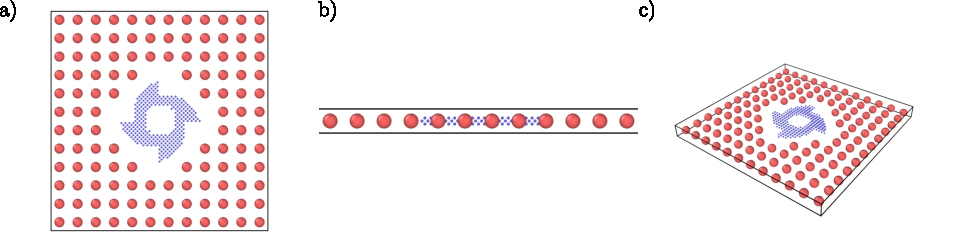
\includegraphics[width=0.95\textwidth]{figures/system.pdf}
  \end{center}
  \caption[System overview.]{System overview for a 4 spikes spin up ratchet at time 0. Panel a) shows the top view. Panel b) show a lateral view. Panel c) shows a perspective view.}\label{fig:system}
\end{figure}



Numerical simulations provide a powerful framework to reproduce and analyze physical phenomena under controlled conditions. Unlike experiments, they allow for precise manipulation of initial parameters, systematic testing of hypotheses, and straightforward replication of results. In particular, simulations are invaluable when dealing with microscopic systems, where stochastic effects and complex interactions can make experimental observations challenging. 


%%%%%%%%%%% New section
Let us first describe the ensemble of paramagnetic colloids. The particles are modeled after Dynabeads M-280 Streptavidin, which possess paramagnetic properties: they acquire a magnetic moment only when an external magnetic field is applied. Once the field is removed, the particles exhibit no remanent magnetization, unlike ferromagnetic materials. The induced magnetic moment aligns instantaneously with the direction of the applied field.
When considering the simplified case of two interacting particles, the dipole–dipole interaction can be either attractive or repulsive depending on their relative orientation, as illustrated in Figure~\ref{fig:pairinteraction}. If the external magnetic field is slowly rotated, the dipoles follow its motion, and the interaction angle between the particles continuously varies from attractive to repulsive, however the average interaction over time is attractive~\cite{massana2019tunable}. There exists, however, a particular angle at which the interaction energy vanishes, it is neither attractive nor repulsive. This critical value is known as the magic angle~\cite{erickson1993magic, hennel2004magic}, given by
\[ \theta = \acos{\frac{1}{\sqrt{3}}} \approx 54.7°.  \]

\begin{figure}
  \begin{center}
    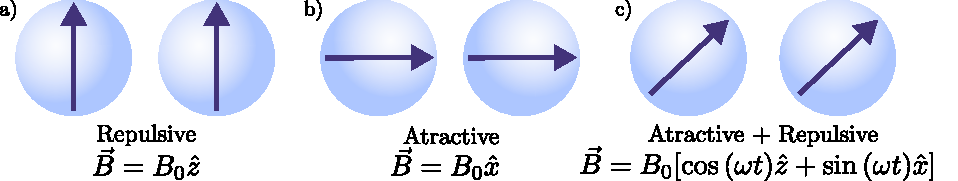
\includegraphics[width=0.95\textwidth]{figures/colloidsdynamics1.pdf}
  \end{center}
  \caption[Basic interaction for a pair of paramagnetic colloids.]{Interaction between a pair of paramagnetic colloids when a) a constant field in $\hat{z}$ is applied, b) constant field in $\hat{x}$ is applied, and c) when a rotating field is applied in the plane $\hat{x}$, $\hat{z}$.}\label{fig:pairinteraction}
\end{figure}

When a pair of particles is placed inside a confined space under a constant magnetic field designed to induce repulsive interactions, the particles will displace from each other until reaching equilibrium. However, when considering the collective dynamics of an infinite chain of particles, where individual displacement is restricted by the presence of neighboring particles, the system instead exhibits vertical motion, as illustrated in Figure~\ref{fig:colloidsconfined}. By varying parameters such as particle packing density and the height of the slit pore~\cite{osterman2007observation}, distinct structural patterns can emerge in the equilibrium configurations. Nonetheless, when the confinement height exceeds a critical threshold, the particles tend to form dimers due to reduced repulsive constraints and enhanced dipolar coupling.

\begin{figure}
  \begin{center}
    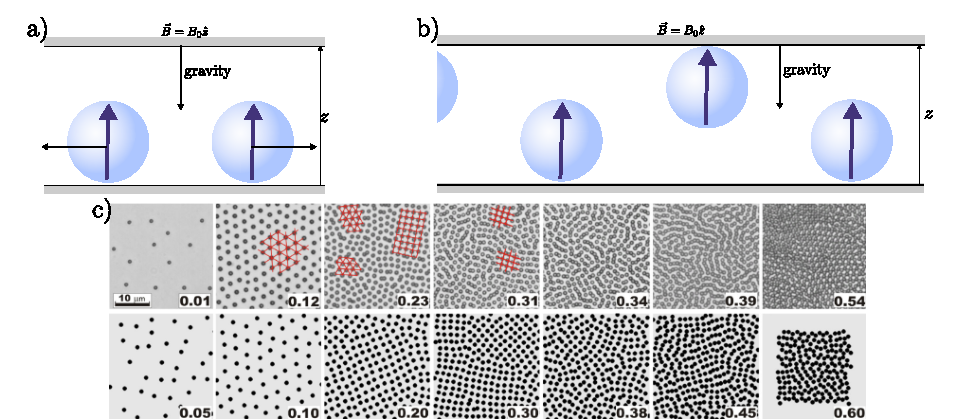
\includegraphics[width=0.95\textwidth]{figures/colloidsdynamics2.pdf}
  \end{center}
  \caption[Dinamycs of paramagnetic colloids in a confined space.]{Dynamics of paramagnetic colloids in confined space in the presence of gravity and a constant field applied in $\hat{z}$ for a) a pair, b) an infite chain. Panel c) shows the behavior of particles at 12.5 mT at different packings, bottom row shows experimental results, bottom row show simulations results, obtained from~\cite{osterman2007observation}.}\label{fig:colloidsconfined}
\end{figure}

Considering the same confined space under the presence of a conical external magnetic field, the dynamics of the colloids vary with the driving frequency. At low frequencies, the particles form pairs (dimers) that rotate synchronously with the magnetic field; this regime is referred to as the synchronous state. At high frequencies, the magnetic torque generated by the dipole interaction becomes smaller than the viscous torque, resulting in a rotational lag. In this regime, the dimers rotate asynchronously, meaning they still spin but no longer match the field’s frequency. At even higher frequencies, another phase coexists—known as the rupture state—where the colloids cease forming dimers and instead arrange into a crystalline structure.

At intermediate frequencies, a transition state emerges in which the colloids exhibit both synchronous and asynchronous behavior. In this regime, particles periodically rotate, separate, and reattach to different neighbors; this state is referred to as the exchange or neighbor-exchange phase in this thesis. These states depend on several factors, including particle packing density and slit-pore height. Figure~\ref{fig:helenapathphases} illustrates some of these transitions for constant height and packing while varying the driving frequency. The neighbor-exchange state, in particular, displays random, ballistic-like trajectories that contribute significantly to the collective dynamics of the solid ratchet.

\begin{figure}
  \begin{center}
    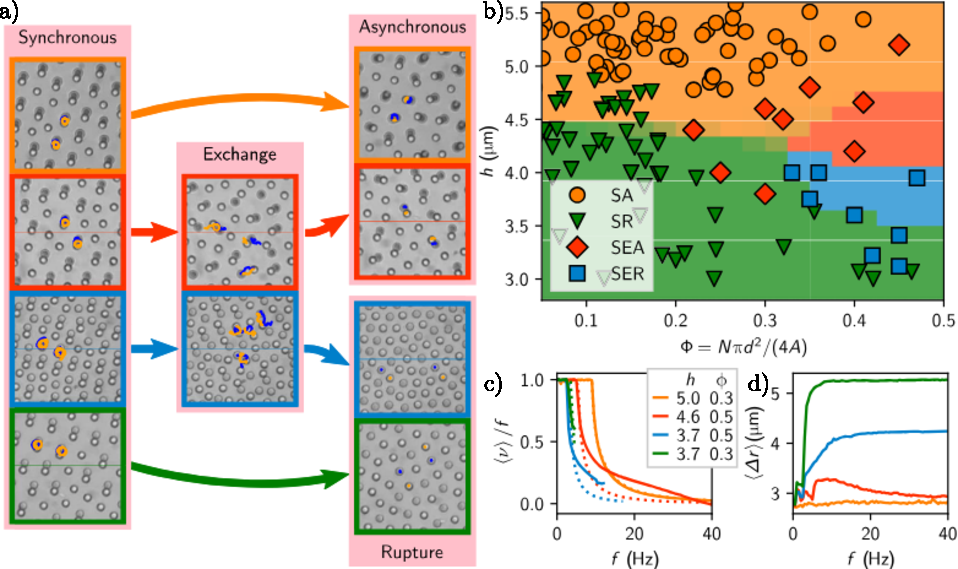
\includegraphics[width=0.95\textwidth]{figures/helenapathphases.pdf}
  \end{center}
\caption[Colloidal states for different packing, height, and frequency.]{Panel a) shows the different phases observed when varying the external magnetic field. The synchronous phase corresponds to particles rotating in phase with the field. In the exchange phase, synchronization with the external field is lost, but particles continue to interact with their neighbors, exchanging positions. The asynchronous phase refers to particles that can no longer follow the external field and instead form dimers. Finally, the rupture phase occurs when particles fail to follow the rotating field but self-organize into a crystalline structure, panel b) shows the location of transition paths deppending on packing and slit pore height. Panel c) shows relative dimer rotation respect to frequency. Panel c) shows the average particle separation respecto to fequency. Obtained from~\cite{massana2020emergent}.}\label{fig:helenapathphases}
\end{figure}

%%%%%%%% End of new section
\section{Molecular Dynamics}

In this thesis, numerical simulations are employed to study the dynamics of colloidal systems at the microscale. Such systems are often dominated by thermal fluctuations and many-body interactions, making them difficult to probe experimentally without advanced imaging and data analysis techniques. The primary computational approach used here is \textit{molecular dynamics} (MD), which will be described in detail in the following sections. MD enables the integration of particle trajectories under the influence of deterministic and stochastic forces, providing direct access to observables such as mean-squared displacements, velocity correlations, and transport coefficients.

This thesis explores the physics of the system by using molecular dynamics, where randomness enters through thermal noise. As we saw in \ref{stochasticrepresentation}, the interactions can be derived from classical mechanics. In this case, Newton’s second law gives the starting point to calculate the forces acting on a single particle. In other words, at each iteration of the simulation we need to evaluate the forces that each particle experiences. Taking equation~(\ref{eq:newton}) as a starting point, and adding labels for the different interactions, we obtain:

\begin{equation}
  m\ddot{\vec{x}} = F^{collision}_i + F^{drag}_i + \eta(t)\text{,}
  \label{eq:langevinratchet}
\end{equation}
where $m_i$ is the mass of particle $i$, $\vec{x_i}$ its position, and $F^{drag}_i$ is the viscous force, written as $-\gamma \dot{\vec{x}}_i$, with $\gamma$ the drag coefficient of the fluid. Since we are working at a scale where inertial effects are negligible, the term $m_i\ddot{\vec{x_i}}$ can be dropped. The random force $\eta(t)$ represents collisions with the solvent particles. In this thesis, $\eta$ is taken as a Gaussian random force with $\expval{\eta} = 0$ and correlation $\expval{\eta_i(t)\eta_j(t')} = 2k_B T \gamma \delta_{i,j}\delta(t-t')$. This form will be used for non-paramagnetic particles.

For paramagnetic particles, we need to add the contribution of dipole–dipole interactions, which gives the modified equation:

\begin{equation}
  0 = F^{collision}_i + F^{drag}_i + F^{dd}_i + \eta(t)\text{,}
  \label{eq:langevindipole}
\end{equation}
where $F^{dd}_i$ according to \cite{yung1998analytic} is described as force exerted for the dipole moment $\vec{m}_i$ on a dipole $\vec{m}_j$:

\begin{equation}
  \label{eq:dipoledipoleforce}
\vec{F}^{dd}_i = \frac{3\mu_0}{4\pi r^4}
\begin{multlined}[t]
\bigl[ (\hat{x}_{i,j} \times \vec{m}_i) \times \vec{m}_j
    + (\hat{x}_{i,j} \times \vec{m}_j) \times \vec{m}_i \\
    - 2\hat{x}_{i,j}(\vec{m}_i \cdot \vec{m}_j)
    + 5\hat{x}_{i,j}((\hat{x}_{i,j} \times \vec{m}_i) \cdot (\hat{x}_{i,j} \times \vec{m}_j)) \bigr],
\end{multlined}
\end{equation}
where $\hat{x}_{i,j}$ is the unitary vector of distance between dipoles. Since all magnetic dipoles are identical and aligned with the external magnetic field $\vec{B}_{\text{ext}}$, we can express the dipole moment as $\vec{m} = \chi V \vec{H}_{\text{ext}} = \frac{\chi V}{\mu_0} \vec{B}_{\text{ext}}$, where $\chi$ is the magnetic susceptibility and $V$ is the particle volume. Substituting $\vec{m}_i = \vec{m}_j = \vec{m}$ and expressing in terms of the external field gives:

\begin{equation}
  \label{eq:dipoledipoleforce_Bext}
  \vec{F}^{dd}_{i,j} = \frac{3\mu_0 m^2}{4\pi r^4}
\left[ 2(\hat{x}_{i,j} \times \hat{B}) \times \hat{B} - 2\hat{x}_{i,j} + 5\hat{x}_{i,j}|\hat{x}_{i,j} \times \hat{B}|^2 \right],
\end{equation}
where $m = \frac{\chi V B_{\text{ext}}}{\mu_0}$, $\hat{B} = \vec{B}_{\text{ext}}/B_{\text{ext}}$ is the unit vector along the external field, and $B_{\text{ext}} = |\vec{B}_{\text{ext}}|$. 

This is the force applied by one particle, to obtain the total dipole interaction with all particles of the system, we should add them up, pair by pair:

\begin{equation}
  F^{dd}_i = \sum^{n}_{i \neq j} F^{dd}_{i,j}.  
  \label{eq:dipolesum}
\end{equation}

We need to define the external magnetic field, which is a precessing field that forms a conical rotation of the form

\begin{equation}
  \vec{B} = B_0 [\cos{\theta}\hat{z} + \sin{\theta}\cos{(\omega t)}\hat{x} + \sin{(\omega t)}\hat{y}],
  \label{eq:magneticfield}
\end{equation}


where $B_0$ is the amplitude and $f$ the frequency of rotation of the magnetic field. The frequency plays an important role in the system dynamics. Depending on how fast the field rotates, it determines whether the internal magnetic dipole of each particle can follow it or not. At low frequencies, the dipoles rotate synchronously with the field, resulting in purely attractive or repulsive interactions. At higher frequencies, however, the dipoles cannot keep up, leading to a phase delay. In this regime, particles can exchange neighbors as the field continues to rotate.


\begin{figure}[H]
  \begin{center}
    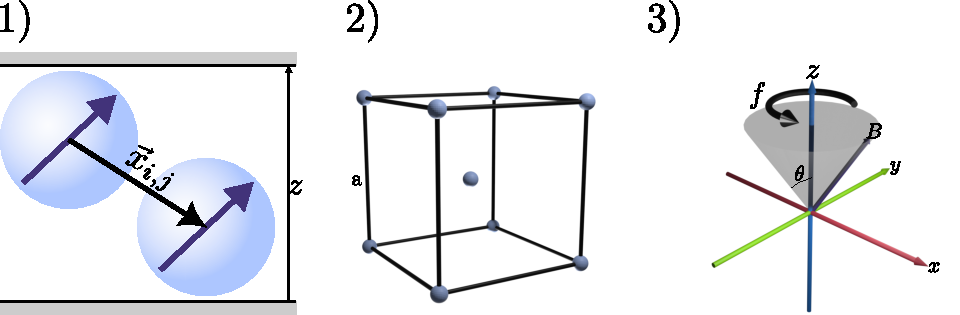
\includegraphics[width=0.95\textwidth]{figures/methods1.pdf}
  \end{center}
  \caption[Representation of the paramagnetic colloids, body-centered-cubic lattice used for the ratchet, and the precessing conic magnetic field.]{Panel a) Shows two paramagnetic particles with a distance \(\vec{x}_{i,j}\) with the same dipole moment in a confined space in the \( z\) axis. Panel b) Shows a representation of a  unitary body-centered cubic lattice used in the construction of the ratchet. Panel c) Shows the precessing external magnetic field used in the simulation.}\label{fig:facecenteredlattice}
\end{figure}

To model contacts, we use a Weeks-Chandler-Andersen potential (WCA), which is a LJ with only a repulsive part~\cite{hess1999augmented}:

\begin{equation}
  U_{i,j}^{WCA} = \begin{cases} 
    4\epsilon\left[ \left( \frac{\sigma}{r_{i,j}}\right)^{12} - \left( \frac{\sigma}{r_{i,j}}\right)^6\right] + \epsilon \quad &r_{i,j} \leq r_c \\
    0 \quad & r_{i,j} \geq r_c
  \end{cases}
  \label{eq:wcapotential}
\end{equation}
where $\sigma$ is the van der Waals radio, it is the point where the energy between the two particles is zero, $\epsilon$ is the well depth, since WCA does not have an attraction interaction, a correction factor of $\epsilon$ is added, and $r_c = 2^{1/6}\sigma$. This however, gives us the enegy between particles, and we need the force, then we apply:

\begin{equation}
 F = - \nabla U, 
  \label{eq:negativegradient}
\end{equation}
getting then

\begin{equation}
  F_{i,j}^{WCA} = \begin{cases} 
    48\epsilon\left[ \left( \frac{\sigma}{r_{i,j}}\right)^{12} - \frac{1}{2}\left( \frac{\sigma}{r_{i,j}}\right)^6\right]\left[ \frac{1}{r_{i,j}}\right] \quad &r_{i,j} \leq r_c \\
    0 \quad & r_{i,j} \geq r_c
  \end{cases}.
  \label{eq:wcaforce}
\end{equation}
and adding all the interaction expected by each particle, we obtain:

\begin{equation}
  F^{collision}_i = \sum^{n}_{i \neq j} F^{WCA}_{i,j}.  
  \label{eq:wcasum}
\end{equation}

We want to see how the positions of the particles evolve over time with certain initial conditions, and to solve Eq. (\ref{eq:langevindipole}) this is why we need an integration method.

\section{Euler-Maruyama Integration Method}
%%%%%%%%
The Euler-Maruyama is a numerical method used for stochastic differential equations which helps solve systems with Brownian motion~\cite{platen2010numerical,higham2001algorithmic}.

The overdamped Langevin equation for a particle reads
\[
  \dot{x}(t)= \frac{1}{\gamma} F(x,t)+\sqrt{2D}\,\eta(t),
\]
where $\gamma$ is the dynamic viscous drag, \(D=k_BT/\gamma\) the diffusion coefficient,
and \(\eta(t)\) is normalized Gaussian white noise:
\(\langle\eta_i(t)\rangle=0,\ \langle\eta_i(t)\eta_j(t')\rangle=\delta_{ij}\delta(t-t')\).
Discretizing with timestep \(\Delta t\) and Wiener increments \(\Delta W\sim\mathcal N(0, 1)\),
the Euler--Maruyama update is
\begin{equation}
x_{n+1} =  x_n + \mu\, F( x_n,t_n)\,\Delta t
  + \sqrt{2D \Delta t}\;\Delta W_n.
\label{eq:em_overdamped}
\end{equation}
%%%%%%%%
\section{Definition of the Solid Ratchet}

To create the solid ratchet we used basis vectors (or lattice vectors) which are the fundamental building blocks used to generate the entire crystal lattice by translation. These vectors define the geometry of the unit cell, and by repeating the unit cell across space, we can form the overall lattice structure. Here, a body-centered cubic (BCC) lattice was chosen since the stability which proved to be stable under thermal fluctuations.
The conventional unit cell for a BCC lattice is a cube with a lattice point at each corner and one at the body center. The vectors defining this cube are simple, orthogonal, and given by:
%
\begin{equation}
  \vec{R} = m(a\hat{x}) + n(a\hat{y}) + p(a\hat{z}) + \delta \frac{a}{2}(\hat{x} + \hat{y} + \hat{z}); \quad m,n,p \in \mathbb{Z},
\end{equation}
%
where \( a \) is the lattice constant (the side length of the cube), and $\delta$ is either 0 or 1, depending if we are refering to the centered particle. Once defined the basis vectors, with help of a script we enter the required parameters that will define the size of the solid ratchet that is defined by a modulated radius function that creates $N$ teeth around the azimuthal direction. The angular coordinate $\phi \in [0, 2\pi)$ is traced in the Cartesian coordinates (x, y).
%%%%
\begin{equation}
R(\phi) = R_0 + A \cdot S\left(\frac{f\phi}{2\pi}\right) - \frac{A}{2}
\end{equation}

where $S(x)$ is the sawtooth function, $A$ is the amplitude of the sawtooth, $f$ the number of complete sawtooth cycles in the circle, $R_0$ base radius of the ratchet profile:

\begin{equation}
S(x) = \begin{cases}
1 - (x \bmod 1) & \text{Spin up} \\
x \bmod 1 & \text{Spin down}
\end{cases}
\end{equation}

Points $\mathbf{r} = (x, y, z)$ are included when $\sqrt{x^2 + y^2} \leq R(\phi)$.
However, these points must remain fixed, otherwise these would separate from each other dissolving the structure, therefore we add bonds.
There are multiple methods to model the potential energy of a bond, the easiest way is to use the harmonic potential that mimics the behavior of a ideal spring and is modeled after Hooke's law:

\begin{equation}
  U^{H}_{i,j}(\vec{x}_{i,j}) = \frac{1}{2}K(\vec{x}_{i,j} - \vec{x}_0)^2,
\end{equation}
where K is the energy per squared distance, $\vec{x}_{i,j}$ is the distance between particle \textit{i}, and \textit{j}, and $x_0$ is the equilibrium distance point.
%%%%%%%%

\section{System Overview and Workflow}

The simulations of this thesis were performed with an open-source software called LAMMPS (Large-scale Atomic/Molecular Massively Parallel Simulator) developed by Sandia National Laboratories. Its advantage is the high efficiency to run simulatios in parallel, reducing the time required to perform multiple calculations \cite{LAMMPS}. We used a modified version of LAMMPS but created custom input scripts using a Python library. These scripts will atomate the process of the input scritpts that will tell LAMMPS everything about the parameters of our simulation, such as the size of the system, the physical conditions, and how long to run for. After the simulations, we used additional custom scripts with the help of a Python library called Pandas, to analyze the results quickly and efficiently.

\begin{figure}[h]
  \begin{center}
    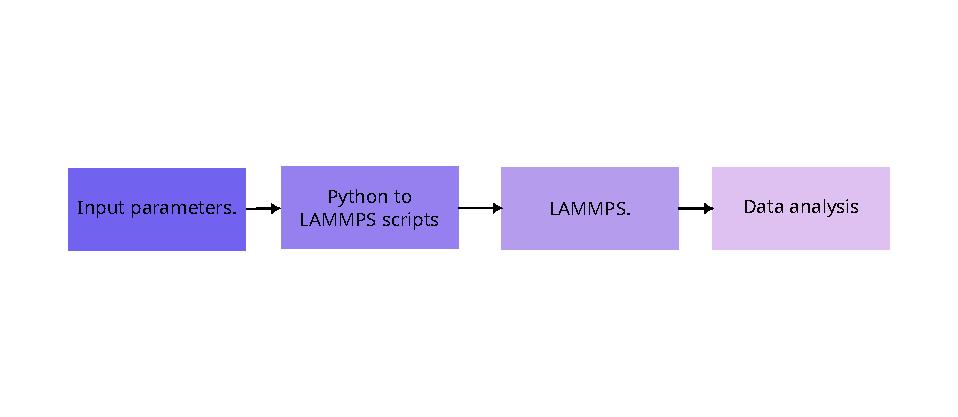
\includegraphics[width=0.95\textwidth]{figures/workflow.pdf}
  \end{center}
  \caption[Workflow diagram.]{Workflow diagram.}\label{fig:workflow}
\end{figure}

\subsection{System's Physical Definition}

The first parameters to be defined are the ones from the circular-ratchet geometry, since it will define the position of the paramagnetic colloids afterwards, these are the parameters that can be specified in the function:

\begin{table}[H]
\centering
\caption[Ratchet physical parameters.]{Parameters used for the circular ratchet in the simulation.}
\begin{tabular}{l l l l l}
\hline
Parameter & Symbol & Ratchet A & Ratchet B & Units \\
\hline
Lattice constant & \(a\) & 1 & 1 & \(\mu m\) \\
Radius & \( r\) & 8 & 8 & \( \mu m\) \\
Sawtooth amplitude & \( A\) & 4 & 4 & \( \mu m\) \\
Sawtooth frequency & \( N\) & 5 & 3 & Dimensionless\\
Bond coefficient & \( K_b\) & 0.1 & 0.1 & \( \mu N\) \\ 
Density & \(\rho\) & 1 & 1 & kgm\(^{-3}\) \\
\hline
\end{tabular}
\end{table}

\begin{figure}
  \begin{center}
    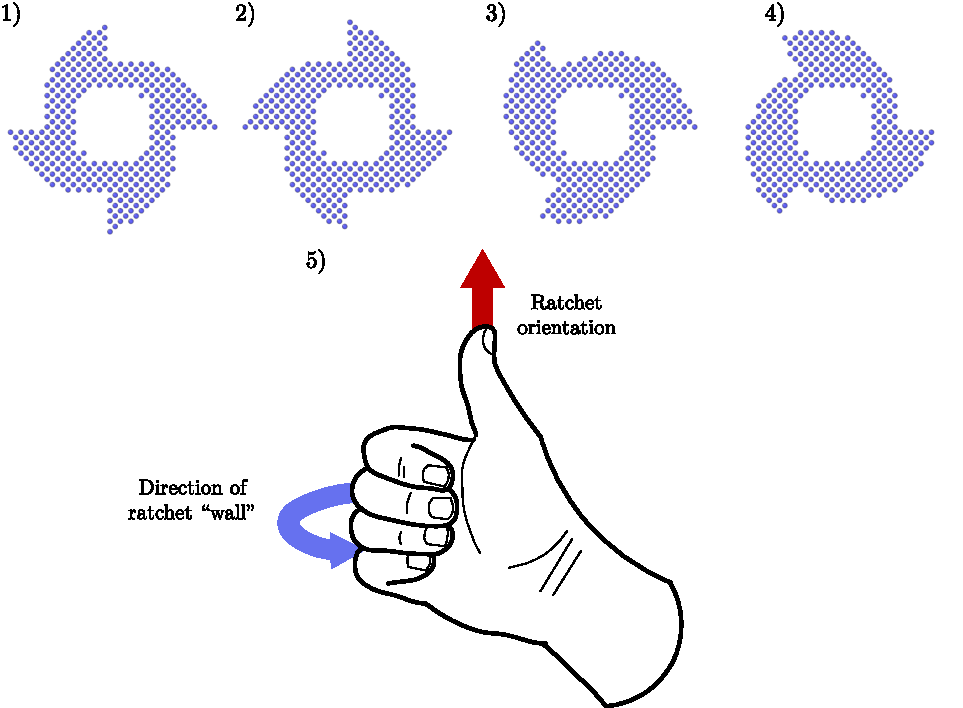
\includegraphics[width=0.95\textwidth]{figures/ratchet.pdf}
  \end{center}
  \caption[Ratchet geomety.]{Ratchet geometry used in the simulations, a) shows 4-spikes ratchet (Spin up). b) shows the same ratchet with a 180° specular rotation (Spin down). Panel c)- d) Shows the same characterisitcs with a 3-spikes ratchet.  Panel b) Shows the convention used for classifying the ratchets. In this case the curl right hand rule can be used. Facing the ``wall'' of the ratchet with the palm of the hand, the thumb will indicate the geometry of the ratchet. If the thumb points towards you or upwards, the geometry will be called spin up, if it points downwards the geometry will be called spin down.}\label{fig:ratchetgeometry}
\end{figure}


As shown in the previous table, there were 2 ratchets with only a difference in te \textit{Sawtooth frequency}, but in reality we used a reflection of each ratchet for another pair of analysis. Once the ratchet geometry is defined, then we can define then the remaining of the system, which remained constant for the 2 ratchets. Starting with the simulation box, that is a rectangle box of periodic boundary conditions in axis \textit{x}, and \textit{y},and finite boundary conditions modeled with the a WCA potential:



\begin{table}[H]
\centering
\caption[Simulation box physical parameters.]{Parameters used for the box of the simulation.}
\begin{tabular}{l l l l}
\hline
Axis & lo  & hi & Units \\
\hline
\textit{x} & -27 & 27 & \( \mu m\) \\
\textit{y} & -27 & 27 & \( \mu m\) \\
\textit{z} & -2  & 2   & \( \mu m\)\\ 
\hline
\end{tabular}
\end{table}

Where \textit{lo} represent the lower boundary, an \textit{hi} the upper boundary.

Finally, the parameters for the paramagnetic particles, and since they deppend on the magnetic field, it is important to define the parameters of this one too.


\begin{table}[H]
\centering
\caption[Paramagnetic colloids parameters.]{Parameters used for the paramagnetic particles.}
\begin{tabular}{l l l l}
\hline
Parameter & Symbol  & Value & Units \\
\hline
Radius & $r_{mag}$ &  1.25 &\( \mu m\) \\
Susceptibility & $\chi$ & 0.4 & Dimensionless\\
Field angle & $\theta$ & 27 & °\\
Frequency & $f$ & [0 - 10] & Hz\\
Field magnitude & $B$ & 7.28 & mT\\
\hline
\end{tabular}
\end{table}

With these values, we can run simulations for a period of $50 \cross 10^6$ frames, with a timestep of 10 $\mu s$ which corresponds to a total real time of $500 s$ ($8.33\bar{3} \mathrm{min})$. Since these systems are of random nature, it is recommended to perform multiple simulations in order to be able to obtain reliable averaged observables, therefore we ran it 10 different times for each frequency.

\subsection{Data Analysis}

%%%%%
When a simulation is completed, LAMMPS generates a text data file containing the quantities selected for output. In this study, we are particularly interested in the particle positions of the solid object, from which several physical properties can be derived—the most relevant being the angular velocity of the ratchet.

The simulated system consists of multiple particles, each exhibiting a slightly different angular velocity due to the bond strength, which prevents them from remaining perfectly rigid with respect to one another. Consequently, it is necessary to compute an average angular velocity that represents the collective motion of all particles.

Since all particles share the same center of mass, the angular velocity can be determined by first calculating this common center, defined as follows:
%%%%%

\begin{equation}
  (x_{\mathrm{COM}}, y_{\mathrm{COM}}) = \displaystyle\frac{\sum^{n}_{i=1} m_i * r_i}{\sum^{n}_{i=1} m_i},
  \label{eq:centerofmass}
\end{equation}
being $m_i$ the mass of the particle \textit{i}, and $r_i$ the position of the particle respect a frame of reference. The best way to calculate the angular velocity is by using polar coordinates, once we have the center of mass, we convert the positions to polar coordinates:

\begin{align}
  r_i & = \sqrt{(x - x_{\mathrm{COM}})^2 + (y - y_{\mathrm{COM}})^2},\\ 
  \theta _i &= \arctan{\frac{y - y_{\mathrm{COM}}}{x - x_{\mathrm{COM}}}},
\end{align}
then we can calculate the angular velocity of each particle for each timestep of the simulation:
\begin{equation}
  \omega _i = \frac{\Delta \theta _i}{\Delta t},
  \label{eq:angularvelocity}
\end{equation}

then obtaining an average angular velocity of all particles. We average over all particles to obtain the angular velocity of the solid object.

